\documentclass[9pt]{article}    
    \usepackage[utf8]{inputenc}
    \usepackage{graphicx}
    \usepackage{float}
    \usepackage[margin=3cm]{geometry}

    \title{\vspace{-4.0cm}COMP47480 Artefact for Practical 3}
    \author{Sukrat Kashyap (14200092)}
    \date{27 February 2018}
    \setlength{\parindent}{0cm}
    \setlength{\parskip}{0.6em}
     
\begin{document}
\maketitle

\section{Iteration 1}

\begin{figure}[htb]
    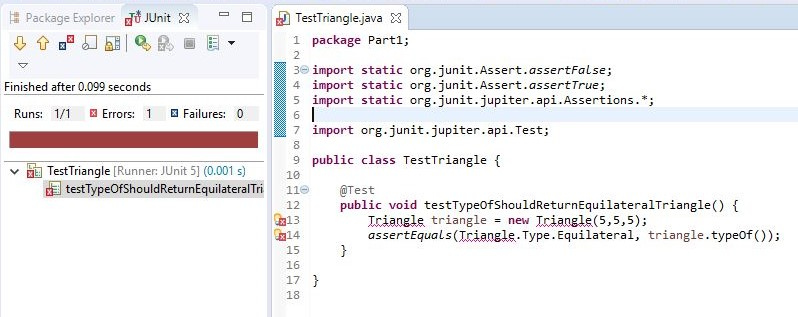
\includegraphics[width=\linewidth]{./pics/p1.JPG}
    \caption{(Failing) Test for equilateral triangle}
\end{figure}

\begin{figure}[htb]
    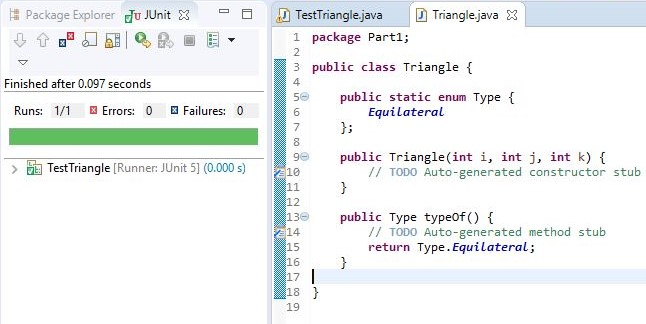
\includegraphics[width=\linewidth]{./pics/p2.JPG}
    \caption{(Passing) Test by adding the production code for equilateral triangle}
\end{figure}

\clearpage{}

\section{Iteration 2}

\begin{figure}[htb]
    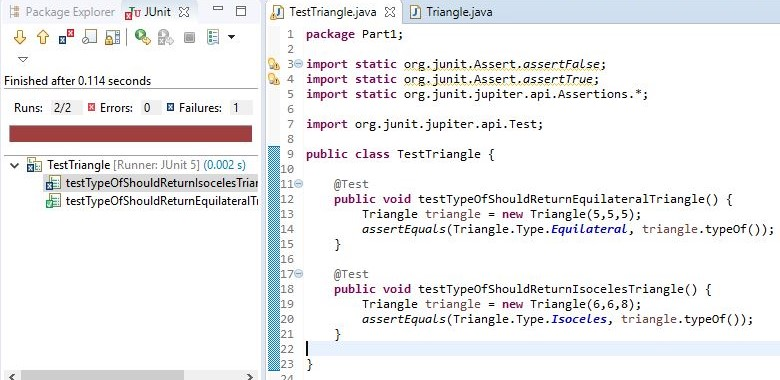
\includegraphics[width=\linewidth]{./pics/p3.JPG}
    \caption{(Failing) Test for isoceles triangle}
\end{figure}

\begin{figure}[htb]
    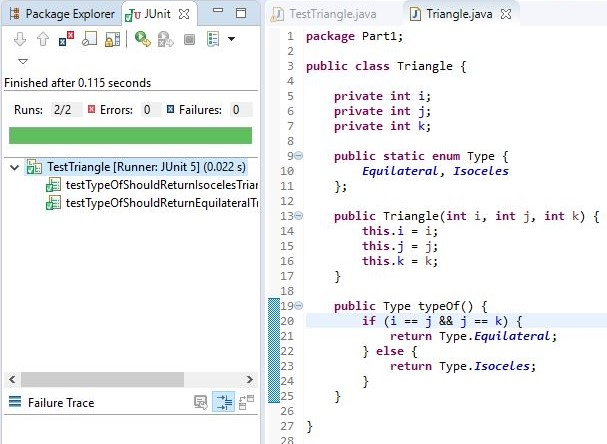
\includegraphics[width=\linewidth]{./pics/p4.JPG}
    \caption{(Passing) Test by adding the production code for isoceles triangle}
\end{figure}

\clearpage{}

\section{Iteration 3}

\begin{figure}[htb]
    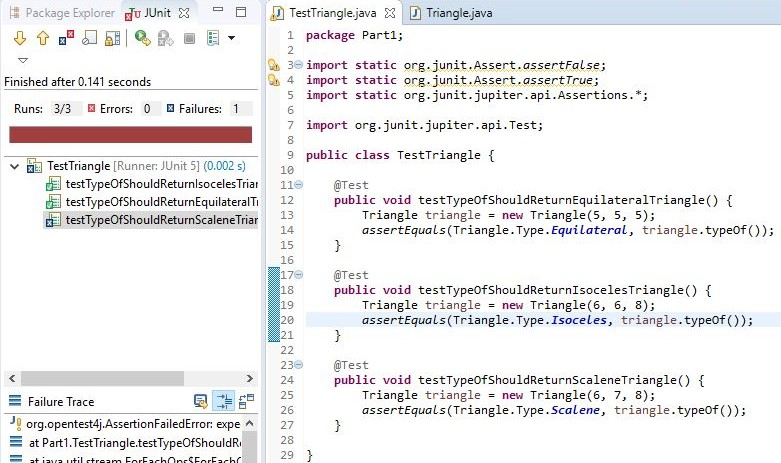
\includegraphics[width=\linewidth]{./pics/p5.JPG}
    \caption{(Failing) Test for scalene triangle}
\end{figure}

\begin{figure}[htb]
    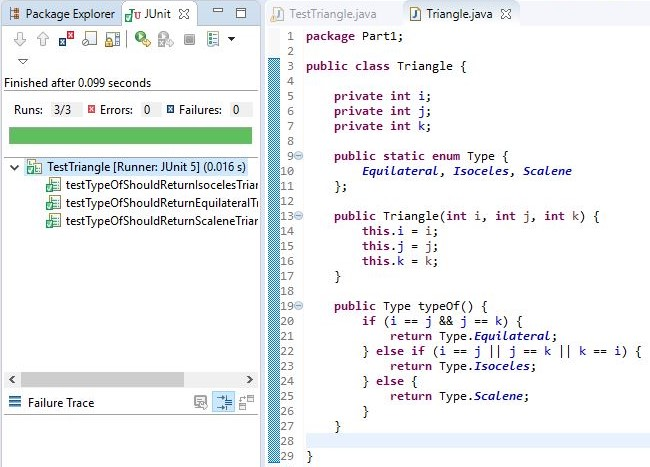
\includegraphics[width=\linewidth]{./pics/p6.JPG}
    \caption{(Passing) Test by adding the production code for scalene triangle}
\end{figure}

\clearpage{}

\section{Iteration 4}

\begin{figure}[htb]
    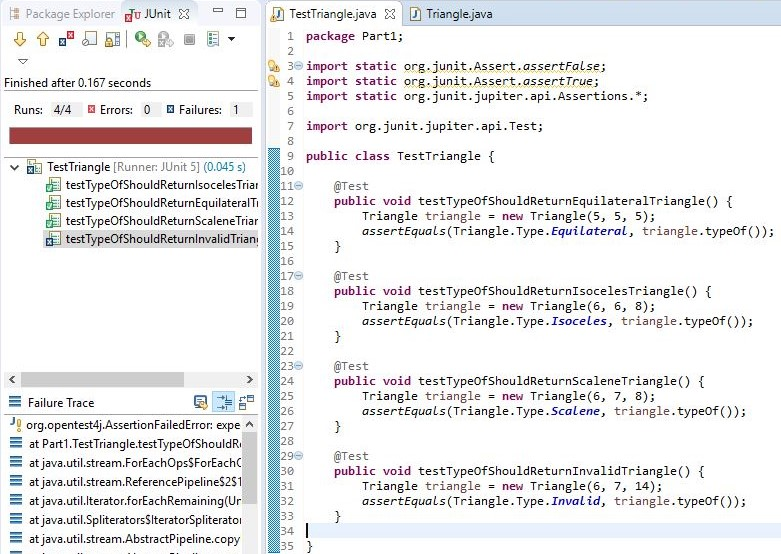
\includegraphics[width=\linewidth]{./pics/p7.JPG}
    \caption{(Failing) Test for invalid triangle}
\end{figure}

\begin{figure}[htb]
    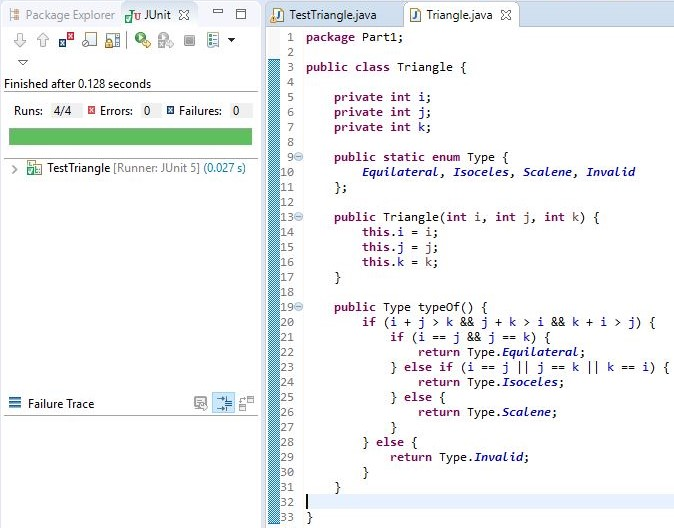
\includegraphics[width=\linewidth]{./pics/p8.JPG}
    \caption{(Passing) Test by adding the production code for invalid triangle}
\end{figure}

\clearpage{}

\section{Iteration 5}

\begin{figure}[htb]
    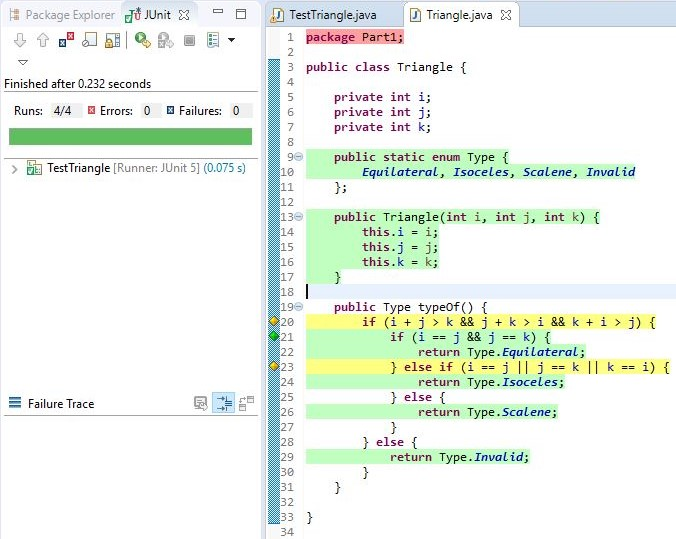
\includegraphics[width=\linewidth]{./pics/p9.JPG}
    \caption{Code coverage: One can see now few branches were not tested}
\end{figure}

\begin{figure}[htb]
    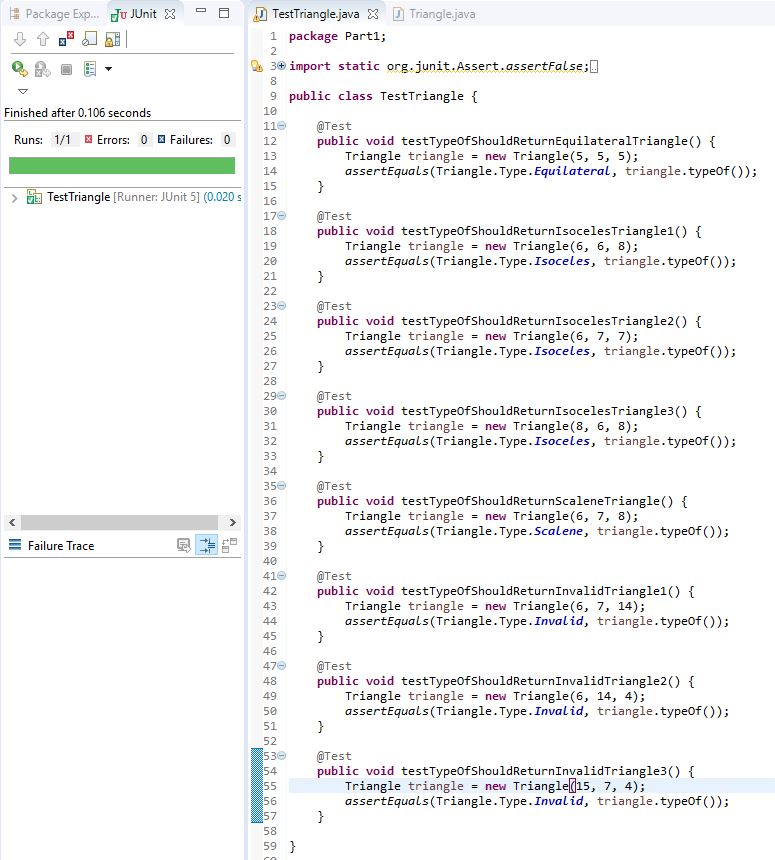
\includegraphics[width=\linewidth]{./pics/p10.JPG}
    \caption{Added code to test the other branches of the production code mainly for isoceles and invalid triangle}
\end{figure}

\begin{figure}[htb]
    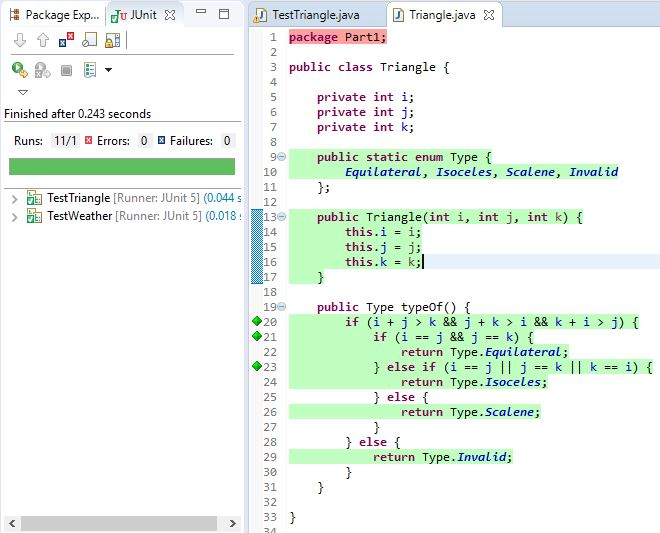
\includegraphics[width=\linewidth]{./pics/p11.JPG}
    \caption{Test show full coverage after the adding the test. *Red colour is because of package issue in the environment}
\end{figure}

\end{document}
